\documentclass[runningheads]{llncs}
%
\usepackage{graphicx}

\begin{document}
%
    \title{AAQC - Autonomous air quality control}

%\author{Smart Cities and Internet of Things - Group 16: \\
%Tobias Haller (\texttt{3132111}) \email{st141219@stud.uni-stuttgart.de}\\
%Jonas Hofer (\texttt{XXXXXXX}) \email{st173462@stud.uni-stuttgart.de} \\
%Christian M\"uller (\texttt{3132108}) \email{st140956@stud.uni-stuttgart.de}}

    \author{Group 16 - Tobias Haller \and Jonas Hofer \and Christian M\"uller}

    \institute{Service Computing Department, IAAS, University of Stuttgart}

%
    \maketitle              % typeset the header of the contribution
%
%\begin{abstract}
%    The abstract should briefly summarize the contents of the report in
%    150--250 words. 
%    
%    \keywords{First keyword  \and Second keyword \and Another keyword.}
%\end{abstract}


    \section{System Introduction}

    Increasing people's efficiency and comfort is an important topic of research.
    Making everyday life more comfortable and easier is a predominant aspect of development related to smart buildings and especially smart homes.
    Therefore, it is not surprising that companies offering solutions for smart cities and smart home devices have significant market growth.

    Since we are participating in the lecture "Smart Cities and IoT" we want to gain practical experience in addition to the theoretical fundamentals taught by the lecture.
    Since Smart Cities are just a bigger model or a further development of a smart home system, we will consider a smart home system as our project.

    Let's assume we live in an appartement with e.g. a kitchen, a bathroom, a living room and a bedroom.
    Since we have a huge music affinity we want to listen the whole day to music while moving in our appartement.
    Without any smart home functionality we would have to turn on the speakers in the room we are currently in or turn it off once again when leaving.
    Additionally, of course we would have to connect our smartphone to some speaker first and play our favorite music.
    Once we got established the connection and the music is playing we would have to regulate the volume of the music according to many factors such as noise in the room.

    In the following based on this basic problem definition and main scope of our work we want to specify our use cases and requirements for a smart home system which aims to automate such tasks as well as some additional ones for a user.


    \section{System Analysis}
    There are some core requirements and functionalities a user wants from this smart home system.
    Given the described scenario we want to improve a users situation by providing a way to play their favorite music in every room where people are currently in.
    In addition we want to extend comfort by increasing and decreasing the volume of the music according to external factors, e.g. the noise in the environment.
    Another part of our smart home system can be to identify the mood of a user and adapt music and environment according to this.

    The core system functions will be separated into both functional and non-functional requirements according to ISO 25010. All requirements will be priorized by - - / - / 0 / + and ++, where all requirements with + or ++ are considered to be mandatory for our project. All other requirements are considered as desirable or optional requirements.

    \subsection{Functional Requirements}

    \begin{description}
        \item[Name] FA-1
        \item[Title] Autonomous temperature regulation
        \item[Description] The system should be able to regulate the temperature of the room based on system information and human presence
        \item[Dependencies] FA-8 FA-10
        \item[Priority] +
    \end{description}

    \begin{description}
        \item[Name] FA-2
        \item[Title] Autonomous humidity regulation
        \item[Description] The system should be able to regulate the humidity of the room based on system information and human presence
        \item[Dependencies] FA-9 FA-10
        \item[Priority] +
    \end{description}

    \begin{description}
        \item[Name] FA-3
        \item[Title] Autonomous air quality regulation
        \item[Description] The system should be able to regulate the air quiality of the room based on system information and human presence. Particle count (Particulate matter) and $CO_2$ concentration are the basis for measuring the air quality.
        \item[Dependencies] FA-6 FA-7 FA-10
        \item[Priority] ++
    \end{description}

    \begin{description}
        \item[Name] FA-4
        \item[Title] Night regulation
        \item[Description] The System should reduce its functionality to a minimum during night time.
        \item[Dependencies] FA-1 FA-2 FA-3
        \item[Priority] 0
    \end{description}

    \begin{description}
        \item[Name] FA-5
        \item[Title] Display system activity to User
        \item[Description] The System should be able to show its activity and monitoring information to the user
        \item[Dependencies] Everything else
        \item[Priority] --
    \end{description}

    \begin{description}
        \item[Name] FA-6
        \item[Title] Recognize stale air
        \item[Description] The System should be able to recognize when the air has gone stale. This is based on the $CO_2$ concentration indoors.
        \item[Dependencies] None
        \item[Priority] ++
    \end{description}

    \begin{description}
        \item[Name] FA-7
        \item[Title] Recognize increased particulate matter concentration
        \item[Description] The System should be able to recognize when the air contains an increased concentration of particulate matter.
        \item[Dependencies] None
        \item[Priority] ++
    \end{description}

    \begin{description}
        \item[Name] FA-8
        \item[Title] Monitor indoor and outdoor temperature
        \item[Description] The System should be able to recognize the temperature indoors and outdoors of its operating location.
        \item[Dependencies] None
        \item[Priority] ++
    \end{description}

    \begin{description}
        \item[Name] FA-9
        \item[Title] Monitor indoor and outdoor humidity
        \item[Description] The System should be able to recognize the humidity indoors and outdoors of its operating location.
        \item[Dependencies] None
        \item[Priority] ++
    \end{description}

    \begin{description}
        \item[Name] FA-10
        \item[Title] Detect human presence
        \item[Description] The System should be able to detect human presence indoors.
        \item[Dependencies] None
        \item[Priority] -
    \end{description}

    \subsection{Non-functional Requirements}

    \begin{description}
        \item[ID] NFA-1
        \item[Title] Realworld application
        \item[Description] The system should be able to be easily transformed to a real world running smart home system.
        \item[Dependencies] None
        \item[Priority] -
    \end{description}

    \begin{description}
        \item[ID] NFA-2
        \item[Title] Automation with minimal user intervention
        \item[Description] The system should utilze AI-planning in order to automate its autonomous functionalities with minimal user intervention.
        \item[Dependencies] None
        \item[Priority] ++
    \end{description}

    \begin{description}
        \item[ID] NFA-3
        \item[Title] Loosely coupled system
        \item[Description] The system should be loosely coupled regarding its communication between devices.
        \item[Dependencies] None
        \item[Priority] ++
    \end{description}

    \section{System Architecture Design}

    In the following we will specify our main components that execute our main functionalities. All components are separated into the following Layers according to ISO/OSI Model.

    \begin{figure}
        \centering
        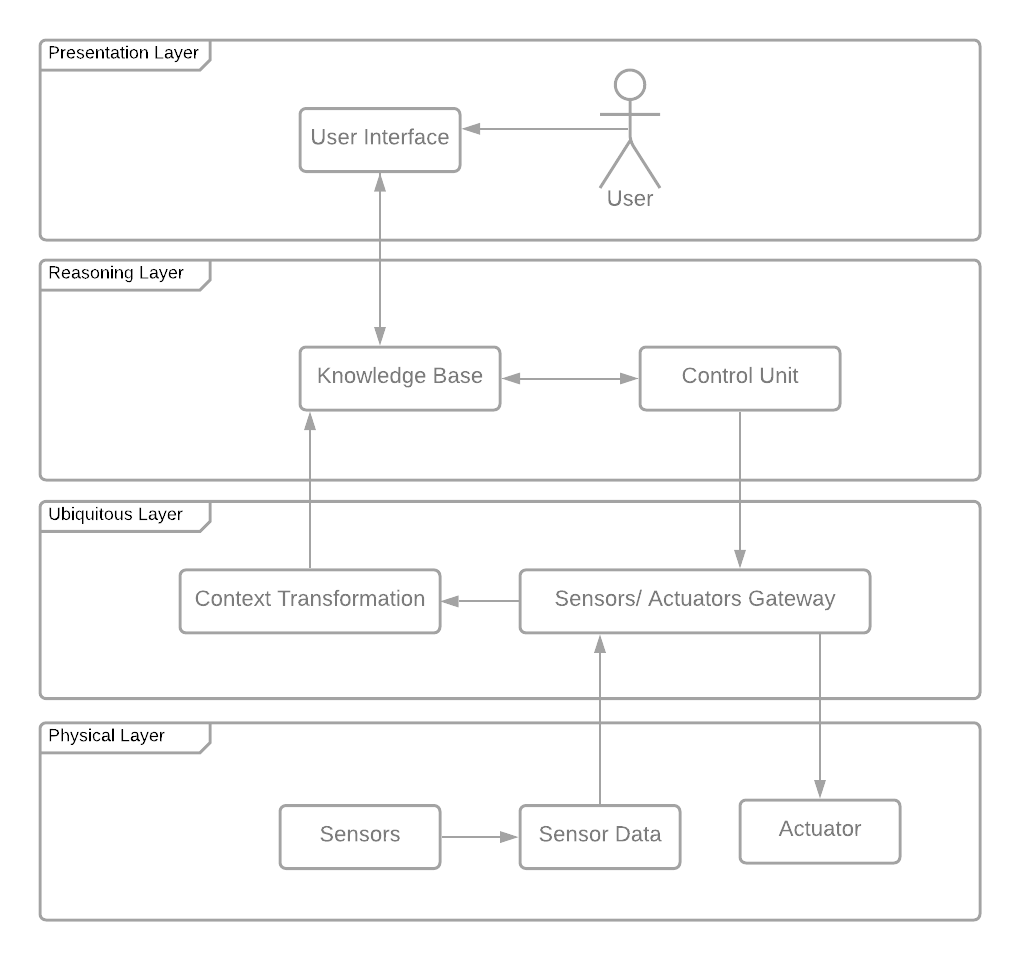
\includegraphics[width=\linewidth]{img/system-design.png}
        \caption{The system design illustrated as a diagram}
        \label{fig:system-design}
    \end{figure}

    \subsection{Presentation Layer}
    The Presentation Layer consists of the User Interface and the User itself. The (human) User interacts with our system via the User Interface which is a GUI. The user can monitor the system as described in functional requirement FA-5.

    \subsection{Reasoning Layer}
    The reasoning layer consists of the knowledge base and the control unit. The knowledge base stores all the sensor data that is generated and stores information about the individual room with the state of all the actuators. It receives all its data from the Context Transformation component in the Ubiquitous Layer. The Control Unit interacts closely with the Knowledge Base, as it receives a notification as soon as new sensor data is stored in the Knowledge Base. Based on all the data, the Control Unit decides based on AI-planning what actions it should take next. As soon as it has reached a conclusion and formulated a plan, it communicates this plan with the Sensors/Actuators gateway in the Ubiquitous Layer.

    \subsection{Ubiquitous Layer}
    The main component of the ubiquitous layer is the sensor/actuator gateway which communicates between the physical layer devices and the components of the reasoning layer. It will process commands from the control unit of the reasoning layer directly in order to relay commands to the actuators of the system. Sensor data however will be given to the Context Transformation component which has the job to take this raw data and transform it to a more precise and informative format which will then be communicated with the knowledge base of the reasoning layer.

    \subsection{Physcial Layer}
    There are two main components of the physical layer. Firstly the sensor which produces sensor data that will be sent to the gateway. Sensors will be used to satisfy functional requirements such as FA-8 and others. Secondly actuators will get instructions from the gateway and execute upon these as is described in the functional requirements.

% \section{System Implementation}
% Describe the implementation of your system. This section is only relevant for the report and should be omitted for the project description. 

% \section{Discussion and Conclusions}
% Here you can discuss some interesting points or limitations of your system and conclude the report.

%
% ---- Bibliography ----
%
%\bibliographystyle{splncs04}
%\bibliography{mybib}

%All links were last followed on \today.

\end{document}
